\documentclass{standalone}
\usepackage{tikz}
\begin{document}
\scriptsize
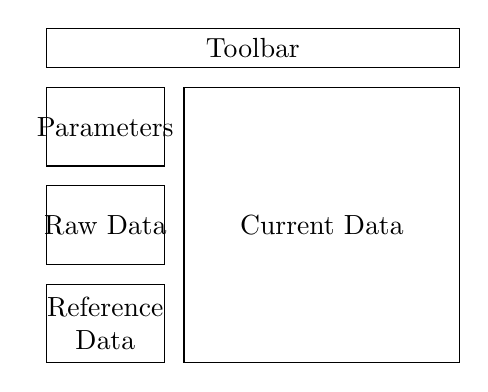
\begin{tikzpicture}[scale=0.5]
  \draw (0,7.5) rectangle ++(10.5,1) node[pos=.5] {Toolbar};
  \draw (0,5) rectangle ++(3,2) node[pos=.5] {Parameters};
  \draw (0,2.5) rectangle ++(3,2) node[pos=.5] {Raw Data};
  \draw (0,0) rectangle ++(3,2) node[pos=.5,align=center] {Reference \\ Data};
  \draw (3.5,0) rectangle ++(7,7) node[pos=.5] {Current Data};
\end{tikzpicture}
\end{document}
